\documentclass[12pt]{article}
\usepackage[utf8]{inputenc} %decia latin1 
\usepackage{amsmath,amsfonts,amssymb,amsthm}
\usepackage[spanish, es-tabla]{babel}
\usepackage[auth-sc,affil-sl]{authblk}
\usepackage[latin1]{inputenc}
\usepackage[spanish]{babel}
\usepackage{graphicx}
\usepackage{natbib}
\usepackage{subfig}
%\usepackage[style=authoryear]{biblatex}
\usepackage[left=2cm,right=2cm,top=2cm,bottom=2cm]{geometry}
\usepackage{setspace}
\usepackage[all]{xy}
%\usepackage{fullpage}
\usepackage{longtable}
%\usepackage {fancyvrb}
\usepackage{fancyhdr}
%\usepackage{color}
\usepackage{pstricks}
\usepackage{amsthm}
%\usepackage{harvard}
\usepackage{float}
\usepackage{footmisc}
\usepackage{hyperref}
\usepackage{pdflscape}
\usepackage{textcomp}
\usepackage{xcolor}
\usepackage[table,xcdraw]{xcolor}
\usepackage[backend=bibtex, style=authoryear]{biblatex}
\addbibresource{biblio/biblio.bib}
%\usepackage[]{draftwatermark}
%\SetWatermarkText{24/05/21}
%\SetWatermarkLightness{0.8}
%\SetWatermarkScale{4}
\usepackage{subcaption}
\usepackage{tabularx}
\usepackage[colorinlistoftodos,prependcaption,textsize=tiny]{todonotes}%MONTXO
\newcommand{\duda}[1]{\todo[color=green!40]{#1}}
\newcommand{\sugerencia}[1]{\todo[color=orange!40]{#1}}
\newcommand{\corregir}[1]{\todo[color=red!40]{#1}}

\setlength{\parindent}{0.5cm}
\setlength{\textwidth}{6.3in}
\setlength{\topmargin}{-33pt}
\setlength{\oddsidemargin}{0pt}
\setlength{\evensidemargin}{0pt}
\setlength{\textheight}{8in}

% cosas del authblk
\setlength{\affilsep}{1mm}
\renewcommand\Authfont{\small} %\scshape\normalsize
\renewcommand\Affilfont{\itshape\small}

\renewcommand\Authsep{  }
\renewcommand\Authand{ }
\renewcommand\Authands{ }


% definiciones
\newcommand{\keywordname}{Palabras clave}
\newenvironment{keywords}{%
	\paragraph*{\keywordname: }}%
{}{}
\newcommand{\area}{{\bf Area:} {\sc Métodos Matemático-Cuantitativos.}}%{\small}

%********************************************%********************************************%********************************************

\begin{document}
	
	\thispagestyle{empty} 
\begin{center}
	
\includegraphics[width=1.00\textwidth]{grafi/logo_inst_80.png}
\end{center}

\vspace{0.3 cm}	
%\textcolor{gray}
\begin{center}
	\hrulefill	\\
	\vspace{0.5 cm}
\textbf{\huge \textcolor{gray} {Una Revisi\'on de M\'etodos de Evaluaci\'on Econ\'omica en Salud}}	\\
	\vspace{0.3 cm}
\hrulefill	\\
\vspace{0.5 cm}
\textbf{Joaqu\'in Viola-Chiazzaro}\\
\vspace{0.5 cm}
\textbf{Ram\'on Alvarez-Vaz}\\
\vspace{0.20 cm}

\end{center}
\vspace{0.5 cm}


\begin{center}
	\textbf{\large Preprint\\
\vspace{0.3 cm}
\noindent  \textnumero 4/23 \\
\vspace{0.3 cm}
\large Segundo semestre, 2023\\
%\vspace{0.3 cm}
% ISSN: 1688-6453 
}\\
\end{center}


\begin{center}
	\vspace{0.5 cm}
{\large \textbf{Universidad de la Rep\'ublica.\\Facultad de Ciencias Econ\'omicas y de Administraci\'on,\\
Instituto de Estad\'istica (IESTA)\\
\vspace{0.7 cm}
Montevideo, Uruguay.}}
\end{center}

%\vspace{0.5 cm}


\includegraphics[width=0.15\textwidth]{grafi/licencia.png}
Esta obra est\'a bajo una Licencia Creative Commons Atribuci\'on - NoComercial - CompartirIgual 4.0 Internacional.

\pagebreak
\thispagestyle{empty} 
\vspace{15.5cm}

Forma de citación sugerida para este documento: 
\begin{flushleft}
	Joaqu\'in Viola-Chiazzaro, Ram\'on Alvarez-Vaz,(2023). \textit{Una Revisi\'on de M\'etodos de Evaluaci\'on Econ\'omica en Salud} (Serie Documentos de Trabajo; \textnumero 4/23). Montevideo: Universidad de la Rep\'ublica. Facultad de Ciencias Econ\'omicas y de Administraci\'on, Instituto de Estad\'istica.
	\url{https://www.colibri.udelar.edu.uy/jspui/handle/20.500.12008/10518}\\
    DOI: \url{10.17605/OSF.IO/UM2VR}
\end{flushleft}

\newpage

\setcounter{page}{1} 
\thispagestyle{empty} 

\begin{center}
	\textbf{}
\end{center}


\begin{center}
	Joaqu\'in Viola-Chiazzaro \footnote{\emph{email: }\texttt{joaquin.viola@fcea.edu.uy}, ORCID: \url{https://orcid.org/0009-0007-4385-9893}\label{fn:foot_autor1}};Ram\'on Alvarez-Vaz \footnote{\emph{email: }\texttt{ramon.alvarez@fcea.edu.uy }, ORCID:\url{https://orcid.org/0000-0002-2505-4238}\label{fn:foot_autor2}}
	\\
	{\small \emph{Departamento de M\'etodos Cuantitativos, Instituto de Estad\'istica, Facultad de Ciencias Econ\'omicas y de Administraci\'on, Universidad de la Rep\'ublica}}
\end{center}
 


\begin{center}
\textbf{Resumen}

\end{center}
En este trabajo se propone hacer una revisión sobre distintos métodos de evaluación económica en la salud, viendo el análisis costo-beneficio y costo-utilidad pero prestando especial interés en el análisis costo-efectividad.
También se hará una breve introducción sobre los distintos aspectos a tener en cuenta a la hora de hacer una evaluación económica, cómo la obtención de los datos sobre los costos de los tratamientos, así como de las medidas de efectividad y su obtención.
Se introducirá el concepto del ratio incremental de costo-efectividad y el incremento del beneficio neto como herramientas para la toma de decisiones.
Se presentarán métodos frecuencistas de intervalos de confianza y métodos de bootstrap para las estimaciones de los parámetros de costos y de efectividad.
Por último se hará una breve presentación de los métodos bayesianos para la evaluación económica de tratamientos médicos.
\\

\begin{center}
\textbf{Abstract}

\end{center}
In this work, we propose to conduct a review of various methods of economic evaluation in healthcare, considering cost-benefit and cost-utility analysis, but with a special focus on cost-effectiveness analysis. We will also provide a brief introduction to various aspects to consider when conducting an economic evaluation, such as obtaining data on treatment costs, as well as measures of effectiveness and how to obtain them. We will introduce the concept of the incremental cost-effectiveness ratio and the increase in net benefit as decision-making tools. We will present frequentist methods of confidence intervals and bootstrap methods for cost and effectiveness parameter estimates. Finally, we will briefly introduce Bayesian methods for the economic evaluation of medical treatments.


\vspace{0.5cm}\\
\textbf{Palabras clave}: Economía de la Salud; Evaluación Económica en Salud; Análisis Costo-Efectividad; Sistema Sanitario; Análisis Bayesiano; Inferencia Estadística.
\vspace{0.5cm}\\ %en orden alfabético 
\textbf{C\'ODIGOS JEL}: C11, C14, D61, H51, I18, I19, .
\vspace{0.5cm}\\
\textbf{Clasificaci\'on MSC2010}: 62P20 .




%\newpage
%\thispagestyle{empty} 
%
%\begin{center}
%	\textbf{ABSTRACT}
%\end{center}
%
%\vspace{0.5cm}\\
%\textbf{Key words}: .
%\vspace{0.5cm}\\
%\textbf{JEL CODES}: .
%\vspace{0.5cm}\\
%\textbf{Mathematics Subject Classification MSC2010}:.
\pagebreak


\pagestyle{fancy}
\fancyhf{}
\fancyhead[RE,LO]{}
\fancyhead[LE,RO]{\thepage}
\fancyfoot[RE,RO]{Viola-Chiazzaro, Joaquín y \'Alvarez-Vaz, Ramón }
\fancyfoot[LE,LO]{DT (4/23) - Instituto de Estadística}

%\maketitle
\tableofcontents
		

\newpage

 

%En una segunda instancia, buscaremos implementar métodos Bayesianos para el análisis de costo-efectevidad, siguiendo algunos resultados del libro "Bayesian Methods in Health Economics" de Gianluca Baio (\cite{baio_bayesian_nodate}), y se usarán datos y códigos de R planteados en "Bayesian Cost-Efectivenness Analysis with the R Package BCEA" del mismo autor (\cite{baio_bayesian_2017}).

    

\subsubsection{Aplicación Análisis Costo-Efectividad en dos tratamientos}

En esta sección usaremos un ejemplo del libro de Elías Moreno \textit{``Bayesian Cost-Effectiveness Analysis of Medical Treatments"}(tabla \ref{tabla:1}), en dónde tenemos los costos y la efectividad promedio de dos tratamientos. (\cite{moreno_bayesian_nodate})

\begin{table}[ht]
\centering
\begin{tabular}{lcc}
  \hline
 & Tratamiento 1 & Tratamiento 0 \\ 
  \hline
Costo Promedio & 7302.70 & 7142.28 \\ 
  Efectividad Promedio (QALY's) & 0.4024 & 0.3958 \\ 
 \hline
\end{tabular}
\caption{Ejemplo 1}
\label{tabla:1}
\end{table}

En el ejemplo obtenemos un incremento del costo de $\$160.42$ y un aumento de la efectividad de $0.0066$ QALY'S al pasar del tratamiento $0$ al tratamiento $1$.
\
De esta forma $\widehat{ICER_{1,0}} = \$24306.06$, es decir, por cada año de vida extra ajustado por la calidad, se tiene un costo de $\$24306$.

\

En este ejemplo, si la disposición a pagar es de \$20000 por una unidad extra de efectividad, no se estaría cambiando al tratamiento $1$, pero para un R de \$25000 si.

\subsubsection{Comparación de más de dos tratamientos}

Ahora supongamos que debemos comparar 5 tratamientos, que todos tienen mayores costos frente a la alternativa de no hacer nada, y también mayor efectividad.\

El concepto de \textbf{dominancia} mencionado anteriormente nos permitirá descartar algunos tratamientos más rápidamente para poder facilitar nuestro análisis. Haremos un gráfico en el plano de los distintos tratamientos, teniendo la efectividad en el eje de las $x$, y los costos en el eje de las $y$. Luego, si el tratamiento ``W'' tiene mayor efectividad y menores costos que ``V'', el tratamiento ``V'' es dominado por ``W'', por lo que podemos descartar a ``V'' cómo nuestra mejor opción. Luego, podemos estar frente a casos en los que no haya una dominancia clara, pero si que un tratamiento tenga mayores costos que uno, y menor efectividad que otro. Como es el caso del tratamiento ``Y'', que tiene mayor costo que ``X'' pero mejor efectividad, y menor costo que ``Z'' y menor efectividad. En este caso decimos que hay una \textbf{dominancia extendida} de ``X'' y ``Z'' sobre el tratamiento ``Y'', porque en la recta que une a ambos tratamientos, hay combinaciones de ambos tratamientos que \textbf{domina} al tratamiento ``Y''. Esto se ve en el gráfico de ``Aplied Methods of Cost-effectiveness Analysis in Health Care" de M.Gray (\cite{gray_applied_2011}).\

Cuando hablamos de dominancia extendida, hay que notar que los tratamientos son mutuamente excluyentes en un paciente, pero no en la población. Para decir existe dominancia extendida de ``X'' y ``Z'' sobre ``Y'' asumimos que en la misma población se puede estar aplicando a una parte de la población el tratamiento ``X'' y a otra parte el tratamiento ``Z'', obteniendo mejores resultados que para el tratamiento ``Y''. La recta que une los puntos ``X'' y ``Z'' es nuestra frontera de costo-efectividad.

\

Veamos el ejemplo del libro de \cite{gray_applied_2011}, para realizar este análisis. Se propone ordenar los tratamientos de forma creciente por sus costos, y luego vamos a ir comparando cada tratamiento con el siguiente de mayor costo, para poder ir eliminando opciones, y poder construir nuestra frontera costo-efectividad.

\begin{table}[H]
\begin{tabularx}{\textwidth}{llllll}
  \hline
Tratamiento & Costos & QALY's & $\Delta_c$ & $\Delta{QALY}$ & ICER\\ 
  \hline
A & 0 & 0 & - & - & -\\ 
B & \$10.000 & 0,4 & \$10.000 & 0,4 & \$25.000 \\
C & \$22.000 & 0,55 & \$12.000 & 0,15 & \$80.000 \\
D & \$25.000 & 0,5 & \$3.000 & -0,05 & Dominado \\
E & \$40.000 & 1 & \$15.000 & 0,5 & \$30.000\\
 \hline
 \end{tabularx}\\
 Se elimina el tratamiento D por ser Dominado por C\\
 \centering
 \begin{tabularx}{\textwidth}{llllll}
 \hline
 Tratamiento & Costos & QALY's & $\Delta_c$ & $\Delta{QALY}$ & ICER\\ 
 \hline
A & 0 & 0 & - & - & -\\ 
B & \$10.000 & 0,4 & \$10.000 & 0,4 & \$25.000 \\
C & \$22.000 & 0,55 & \$12.000 & 0,15 & Dominancia Extendida \\
E & \$40.000 & 1 & \$18.000 & 0,45 & \$40.000\\
 \hline
\end{tabularx}\\

Se elimina el tratamiento C por estar dominado por B y E\\

\centering
\begin{tabularx}{\textwidth}{llllll}
\hline
 Tratamiento & Costos & QALY's & $\Delta_c$ & $\Delta{QALY}$ & ICER\\ 
 \hline
A & 0 & 0 & - & - & -\\ 
B & \$10.000 & 0,4 & \$10.000 & 0,4 & \$25.000 \\
E & \$40.000 & 1 & \$30.000 & 0,6 & \$50.000\\
\hline
\end{tabularx}

\caption{Ejemplo Varios Tratamiento M.Gray}
\label{tabla:2}
\end{table}

\begin{figure}[H]
    \centering
    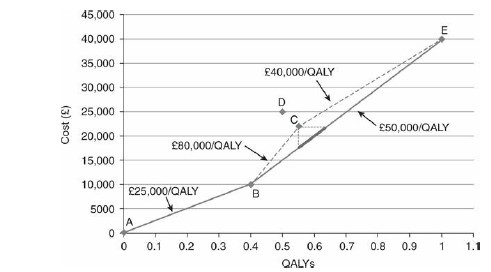
\includegraphics[width=1\textwidth]{grafi/mutuamente_excluyentes_M_Gray.jpg}
    \caption{Plano QALY-Costo de varios tratamientos fuente: M.Gray (2013)}
    \label{fig:2}
\end{figure}



\subsection{Otros Análisis Económicos en Salud}

Como se menciona anteriormente, el análisis de costo-efectividad es el método más usado para la evaluación económica, pero no es el único, también existe el análisis costo-beneficio, minimización de costos. En esta sección buscaremos dar al lector una breve introducción sobre estos métodos.



\section{Fuentes de datos para los análisis económicos en salud}

Los ensayos de control aleatorio son una fuente muy buena para poder comparar los resultados de uno o más tratamientos, pero los agencias regulatorias y la industria de la salud han sumado fuentes extra para mejorar el análisis, como los estudios observacionales. Pero frente a las limitaciones de estas fuentes de datos, debemos tener ciertos cuidados para agregar la información que nos pueden dar para nuestra evaluación. \cite{gray_applied_2011}\\

Para el uso de fuentes de datos y evidencias alternativas podemos encontrar que existe cierta jerarquía .
Una revisión sistemática y el meta-análisis sobre los resultado obtenidos en los ensayos de control aleatorios (RCT's por sus siglas en inglés) encabezan en primer lugar como la mejor fuente de resultados para la evaluación económica, seguido por estudios de cohortes, estudios de control y estudios transversales \cite{alemayehu_statistical_2017}.

\subsection{Ensayos de Control Aleatorio}

Los ensayos de control aleatorio (RCT, por Randomized Control Trials) son los de mayor validez en cuanto a sus resultados, ya que logran que los resultados no se den por la causalidades que llevan a que participantes con similares características conocidads o desconocidas estén en el mismo grupo.\\
Nuestro principal resultado a observar es la diferencia entre el grupo de control y el grupo de tratamiento en el porcentaje de ocurrencia de cierto evento o el tiempo hasta la ocurrencia del mismo.\\

Para la evaluación de drogas, según la ''Food and Drugs Administration'' (\cite{alemayehu_statistical_2017})  los RCT suelen estar separados en distintas fases, con distinta cantidad de pacientes por grupo en cada una '.
En la fase 1 tenemos de 20 a 100 voluntarios durante algunos meses, y se busca ver los posibles efectos adversos que tiene la droga y cómo la droga es metabolizada. En la fase 2, que puede tener una duración de hasta 2 años, con algunos cientos de voluntarios, se obtienen datos preliminares de la eficacia comparada con el grupo de control, y se sigue observando posibles efectos adversos y la seguridad de la droga en el corto plazo.
En la fase 3 participan de 300 a 3000 voluntarios durante 1 a 4 años, a veces de varios países, y busca confirmar los resultados obtenidos y colectar más información sobre la efectividad de los tratamientos a largo plazo. Por último, la fase 4 es luego de la aprovación de la FDA para la comercialización, busca seguir recopilando información sobre la seguridad y los resultados del tratamiento, y obtener recomendaciones para subgrupos de pacientes, cómo diferencias por sexo, o alguna otra característica que los identifique.

\subsection{Estudios Observacionales}

Nos referimos aquellos estudios observacionales a aquellos que no incluyen una posible intervención por parte del investigador. Estos estudios tienen Datos Reales (RWD, por Real World Data) que generan Evidencia Real (RWE, Real World Evidence), suelen ser más fáciles de implementar y tener menos costos. La evidencia puede ser obtenida de la información médica de los registros de salud de los hospitales que contengan registros médicos electrónicos y de facturación.\\
Los datos observacionales se basan sobre base de datos existentes, y nuestra metodología de trabajo variará según el interés de nuestro estudio en particular, algunos estudios observacionales pueden ser estudios de cohortes, estudios transversales o estudios de control de casos. (\cite{alemayehu_statistical_2017})

\subsection{Ensayos Pragmáticos}

Son los tipos de ensayos que más se acercan a nuestro interés para la evaluación económica en salud, mientras los ensayos de control aleatorio ocurren en condiciones experimentales, los ensayos pragmáticos son minimamente controlados, y sirven para medir la efectividad de los medicamentos, así como los costos, es considerado como un estudio observacional especial.

\subsection{Meta-Análisis y Revisión Sistemática}

Es la aplicación de métodos estadísticos para combinar los resultados obtenidos en distintos estudios y poder obtener conclusiones.
El meta-análisis es usado para establecer una diferencia estadística en estudios que tienen resultados conflictivos, para desarrollar una estimación de la efectividad, para tener más información acerca de los daños, los beneficios y la magnitud de los efectos. Un buen trabajo de meta-análisis permite obtener conclusiones y evidencia más fuertes.

\subsection{Búsqueda de Resultados y Costos}

\cite{edlin_cost_2015} Edlin (2015) sugiere el uso de algunas bases de datos de estudios médicos en la web, y también presenta ciertas recomendaciones para tener una búsqueda más efectiva. Existen algunas bases para las que se requieren de permisos institucionales o son pagas, pero entre las bases gratuitas se destaca \textit{PubMed} que es la versión gratuita de MEDLINE (que pertenece a la Biblioteca Nacional de Medicina de Estados Unidos), Embase, Cochrane Library y NHS Economic Evaluation Database.\\

Para facilitar nuestra búsqueda, nos sugieren que planteemos la pregunta sobre la que queremos obtener información, y extraigamos los conceptos claves, para buscar papers y documentos a partir de esto, los motores de búsqueda de la base de datos encontrará los documentos que coincida con todos los conceptos que ingresamos en nuestra búsqueda. Por ejemplo, si queremos buscar trabajos previos sobre el cáncer de mama, y nuestra pregunta es ''¿Qué tan efectiva es la Herceptina en el cáncer de mama?'', nuestras palabras claves serán \textbf{estudios de efectividad}, \textbf{cancer de mama} y \textbf{herceptina}. Si en nuestra base de datos existen 10.000 trabajos sobre estudios de efectividad, 3.000 sobre cancer de mama y 200 sobre herceptina, y solo en 30 trabajos habla de los 3 conceptos a la vez, obtendremos estos 30 trabajos con la información que estamos buscando.\\

Esta técnica se conoce como \textbf{PICO} por sus siglas en inglés (Patient Problem o Population, Intervention, Comparission y Outcomes), que consiste en ingresar en nuestra búsqueda el problema o la población de estudio, la intervención, los métodos de comparación y los resultados, luego, usando el operador lógico ''AND'', buscará documentos que coincida en todo lo que se busca. Se debe tener en cuenta que hay veces que al mimso problema se le llama de diferentes maneras, o son cosas similares que nos puede interesar, cómo puede ser ''cáncer'' y ''tumor'', o ''mama'' y ''pecho'', por lo que podemos agregar el operador lógico ''OR'' para que nos encuentre cualquiera de las combinaciones de la siguiente manera (cáncer OR tumor)AND(mama OR pecho). A continuación podemos ver cómo sería la búsqueda y la cantidad de documentos que se encuentra en Cochrane Library para este ejemplo.

\begin{figure}[htbp]
    \centering
    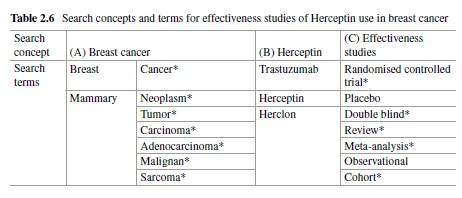
\includegraphics[width=1\textwidth]{grafi/busqueda_cancer_mama.jpg}
    \caption{Ejemplo ''Cost Effectiveness Modelling for Health Technology Assessment'' Richard Edlin, et.al}
    \label{fig:7}
\end{figure}

\begin{figure}[p]
    \centering
    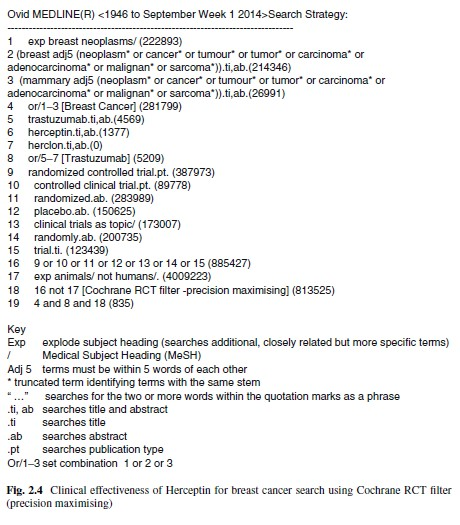
\includegraphics[width=0.75\textwidth]{grafi/resultado_cancer_mama.jpg}
    \caption{Ejemplo ''Cost Effectiveness Modelling for Health Technology Assessment'' Richard Edlin, et.al}
    \label{fig:8}
  
    En la línea 19, vemos que se encontrar 835 documentos con nuestras especificaciones. 
\end{figure}

Por otro lado, para obtener resultados sobre los costos asociados a distintos tratamientos podemos recurrir a algunas de las mismas fuentes que se presentaron anteriormente en esta sección, pero antes, hagamos algunas salvedades sobre los detalles y las diferencias que pueden tener la presentación de los costos en las distintas bases de datos. Los costos asociados a un tratamiento en distintas partes del mundo deberán tener información tanto para la atención pública cómo para la atención privada, también se debe contar con los costos de tarifas médicas, los de testeo, de aplicación y de hospitalización. Cuanto más información tengamos y más detallada esté será mejor, para poder guiar nuestro análisis según nuestros intereses, ya que tal vez no nos interesa agregar algún costo para el análisis que estamos haciendo, o sabemos que el costo en un determinado rubro es considerablemente diferente al de la fuente de donde obtenemos los datos.\\

Algunas de las base de datos de donde podemos obtener datos sobre los costos son: BNF Drug Prices (que contiene precios de drogas en Reino Unido), Canadian Institute for Health Information (CIHI, con datos sobre los costos de procedimientos hospitalarios) y Cost effectiveness Registry

\section{Métodos para Obtener Resultados sobre la efectividad}

En esta sección se presentará cómo utilizar algunos conceptos relacionados al ''Análisis de Supervivencia'', para comparar la supervivencia de dos grupos, en nuestro caso, del grupo que estará con el tratamiento del control, y el grupo que estará con el tratamiento alternativo, y ver que datos nos pueden llegar a interesar de esto para nuestro análisis de costo-efectividad, luego también presentaremos el uso de tablas de mortalidad para la evaluación económica en salud, pero esto cómo un caso más general, en el que podemos tener particular interés de testear políticas públicas, con potencial alcance a toda la población.

\subsection{Análisis de Supervivencia}

En general, el análisis de supervivencia es un estudio para medir las probabilidades de 'falla' durante el tiempo, y por falla podemos pensar en el caso más genérico de fallecer, pero también nos puede interesar la ocurrencia de cierto evento, como puede ser tener un infarto al mio-cardio, sufrir un ACV o volver a fumar, pero en todos los casos, mientras el individuo no sufre uno de estos eventos, diremos que 'sobrevive'. Esto nos motiva a introducir el concepto de 'Función de Supervivencia' ($S(t)$), que depende del tiempo, y no es más que la probabilidad de sobrevivir al tiempo $t$, es decir, siendo $T$ el tiempo de falla, es la probabilidad de que $T>t$ (\cite{gray_applied_2011}).

$$S(t)=P(T>t)$$

Y como toda función de probabilidad, cumple que $S(0)=1$, es decreciente y $S(t)\longrightarrow 0 \text{  cuando  } t \longrightarrow \infty$.\

También contamos con una \textit{funció de riesgo} ($h(t)$), que es la tasa instantánea de falla, al momento t dado que se sobrevivió hasta t.

$$h(t) = lim_{\Delta{t}\longrightarrow 0}\frac{P(t<T<t+\Delta{t}|T>t)}{\Delta{t}}$$

De todas formas, la anterior fórmula es meramente para presentarla, ya que en general trabajaremos con tiempos discretos (como meses o años) y tendremos formas más fáciles de hallar el riesgo para  cada momento. Luego, podremos calcular el riesgo acumulado ($H(t)$) al momento t, mediante integrales, o sumas, depende si estamos en casos continuos o discretos, desde el momento 0 al momento t.

$$H(t) = \int_{0}^{t}h(u)du  \text{  ó  } H(t)=\sum_{u=0}^{t} h(u)$$.

Se puede observar que estas ecuaciones están relacionadas, de forma tal que $H(t)=-L(S(t))$, ó también $S(t) = e^{-H(t)}$. Luego, como esperamos que nuestros tratamientos tengan distinto comportamiento en los riesgos, esperamos ver diferencias en la función de supervivencia. (Para una explicación más detallada de este resultado se sugiere el libro 'Applied Analysis Survival Using R' de Dirgk F. Moore \cite{moore_applied_2016})

\begin{center}
    \textbf{Modelos No Paramétricos}
\end{center}

En primer lugar presentaremos los modelos no paramétricos, que no siguen una forma funcional, y solo se basan en los datos. En estos casos, tendremos funciones de supervivencia discretas, con saltos en cada momento de falla, por lo que el largo de los saltos dependerá de los momentos de fallas, a no ser que contemos las fallas todos los meses, o todos los años, ahí tendremos saltos de igual largo, con la salvedad de que no habrá salto si en un mes no ocurre una falla.\

Nuestra función de supervivencia, al momento t, será el producto de las probabilidad de sobrevivir en cada uno de los momentos anteriores hasta el momento t incluído, así que teniendo las fallas ($d_t$) y los individuos que pueden fallar ($n_t$) en cada momento, nuestra función de supervivencia de \textit{Kaplan-Meier} al momento t es:

$$S(t)=(1-d_1/n_1)(1-d_2/n_2) \dotsb (1-d_t/n_t)$$
$$S(t) = \prod_{t_i\leq t} (1-\frac{d_i}{n_i})$$

Hay que tener cuidado con los valores de $n_t$ en cada momento, ya que no necesariemente es igual al total de la población de estudio menos las muertes hasta el momento anterior. Ya que podemos tener datos censurados. Estos son individuos que no forman más parte de nuestro estudio (ya sea por fallecimiento u otro motivo) pero este fallecimiento no está relacionado con lo que estamos estudiando. Por ejemplo, si estamos testeando un medicamento para prevenir infartos al mio-cardio, y un individuo fallece en un accidente de tránsito, no forma más parte de nuestro estudio, pero el motivo de falla no es de nuestro interés.

\

En los datos que están en el archivo ''SURVIVAL\_DATA.xlsx'', sacados del libro \cite{gray_applied_2011}, tenemos la opción de medir dos cosas distintas, por un lado, el tiempo de fallecimiento, para el cuál tenemos un seguimiento de 40 años, y no tenemos datos censurados, y por otro lado el tiempo de ocurrencia de un cierto evento, que nosotros supondremos que es un ataque al corazón, y podemos suponer que son personas ''propensas'' a sufrir uno, estos asuntos no son el centro de interés de esta sección. Además tenemos información de la edad y el sexo de los individuos (que más adelante en esta sección nos será util), y un identificador de a que grupo pertenece (toma valores 0 y 1), esta variable es la que nos interesará por ahora.\

\begin{table}[ht]
\centering
\begin{tabular}{lrrr}
  \hline
orden & tiempo & censura & trat \\ 
  \hline
1 & 0.03 & 1 & 0 \\ 
  2 & 0.10 & 0 & 0 \\ 
  3 & 0.12 & 1 & 1 \\ 
  4 & 0.15 & 1 & 1 \\ 
  5 & 0.28 & 1 & 0 \\ 
  6 & 0.68 & 1 & 0 \\ 
   \hline
\end{tabular}
\caption{primeras 6 fallas (censura = 1) ó censuras (censura = 0)}
\end{table}

En el archivo ''asuntos\_supervivencia.R'', calcuamos las funciones de supervivencia para dos grupos, con distintos tratamientos, y sus intervalos de confianza, generando el gráfico \ref{fig:7}. Nuestro valor de interés será la esperanza de vida en cada uno de los grupos, calculada cómo el área abajo de cada uno de los gráficos, que al ser gráficos partidos, es la suma de rectángulos, con base igual a la diferencia entre dos tiempos consecutivos, y altura igual a la supervivencia del primero de esos tiempos, ya que la función de supervivencia al ser una distribución de probabilidad, es continua por la derecha.\\

\begin{figure}[H]
    \centering
    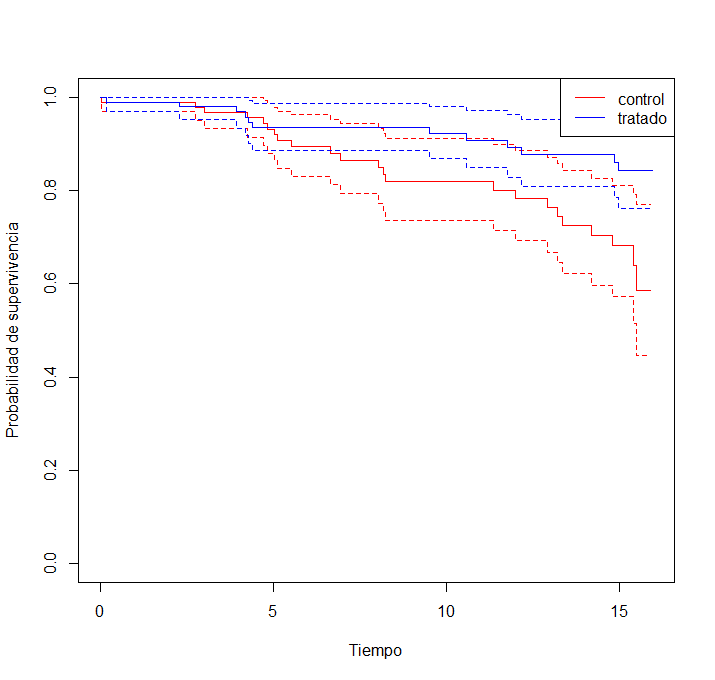
\includegraphics[width=0.8\textwidth]{grafi/supervivencia_dos_tratamientos.jpg}
    \caption{Análisis de Supervivencia de comparación de dos tratamientos}
    \label{fig:7}
\end{figure}

En la tabla \ref{Tabla:8} podemos ver las estimaciones de las esperanzas de vida para el grupo de control y el grupo de tratamiento con sus respectivos intervalos de confianza, obteniendo una diferencia de $2.25$ años en las estimaciones puntuales.

\begin{table}[ht]
\centering
\begin{tabular}{lrrr}
  \hline
 Población & Esperanza & Inf\_95\% & Sup\_95\% \\ 
  \hline
Control & 10.30 & 8.83 & 11.47 \\ 
Tratamiento & 12.55 & 11.15 & 13.50 \\ 
   \hline
\end{tabular}
\caption{Resultados de las esperanzas de vida y los intervalos de confianza al 95\% con el método log-log}
\label{Tabla:8}
\end{table}

\begin{center}
    \textbf{Modelo de Riesgos Proporcionales de Cox}
\end{center}

Estos modelos son modelos semiparamétricos, que cuentan con un riesgo ''base'' $h_0(t)$, y luego las variables de interés de cada individuo forman parte del modelo en forma de covariable, estando el grupo el tratamiento que recibe cada individuo dentro de estas covariables. El riesgo de un individuo queda determinado por $h(t|x_i)=h_0e^{x_i\beta}$, donde en $x_i$ están los valores de las covariables del individuo i, y en $\beta$ los coeficientes asociados al riesgo proporcional de cada covariable, que se calculan mediante máxima verosimilitud.\

Estos modelos nos pueden ser de particular ayuda en el caso en que comencemos con igual cantidad de hombres y mujeres en cada tratamiento, y al final del tiempo de seguimiento veamos una clara diferencia en la proporción de cada sexo que haya sobrevivido, o que no haya sufrido el evento de interés.\

Un valor del coeficiente positivo asociado al sexo masculino indica que el riesgo de los hombres es mayor que el riesgo de las mujeres en cada momento del tiempo. Ya que las covariables son independientes al tiempo. Este influye en el riesgo ''base'' $h_0(t)$.\

Por otro lado, si estamos comparando únicamente dos tratamientos mediante el Modelo de Riesgos Proporcionales de Cox, vemos que $h_0(t)$ es la función de riesgo de para el grupo de control, y $h_0(t)e^{\beta}$ la función de riesgo para el grupo de tratamiento, si queremos queremos que este tratamiento sea mejor que el de control, buscaremos que $e^\beta<1$ es decir, $\beta<0$. Luego, con los resultados mostrados al principio de la sección, donde $S(t)=e^{-H(t)}$ tendremos la función de supervivencia para cada tratamiento. 

\subsection{Tablas de Vida}

Al igual que en los métodos de análisis de supervivencia, el principal interés será en medir la diferencia en las esperanzas de vida de cada grupo y los años de vida ganado.
Las tablas de vida ó mortalidad son ampliamente usada por demografos y actuarios, el desarrollo de estas datan del siglo XVII, donde se construían a partir de los registros de nacimientos y fallecimientos de las iglesias (\cite{gray_applied_2011}).\
Existen dos tipos de tablas de vida, las tablas de vida de cohorte, que mide la supervivencia a lo largo de los años de una cohorte de individuos, pero es muy difícil de aplicar en la realidad por las dificultes para seguir a los individuos a lo largo del tiempo, por lo que se construyen tablas de vida reales o actuales \duda{¿traducción de ''current life table''} con los registros vitales. \duda{¿es necesario explicar las diferencias entre los tipos de tablas de vida}.\\



También pueden estar agrupadas por tramos etareos o bien tener la mortalidad detallada para cada edad puntual, donde se suele tener más detalles en las primeras semanas y meses de vida por el especial comportamiento de la mortalidad en estos momentos. Para la construcción de las tablas de mortalidad se utiliza la experiencia de mortalidad de los últimos años de la población objetivo, y nos permite calcular las tasas de fallecimiento a cada edad, la esperanza de los años de vida restantes y otros datos más. En la Tabla \ref{tabla:6} se encuentra parte de la tabla de mortalidad para los hombres uruguayos en el año 2011.\

Para la construcción de las tablas se suele partir de una cohorte ficticia de 100.000 individuos en la edad 0, y con el pasar de las edades este número irá decreciendo, para la edad x, este valor lo encontramos en la columna de \textit{$l_x$} que indica cuantos individuos tenemos vivos a esas edad. En \textit{$d_x$} tenemos los fallecimientos de la edad x, \textit{$q_x$} indica la tasa de fallecimientos de la edad x $q_x=d_x/l_x$, \textit{$L_x$} son los años vividos por los individuos en la edad x, así, los que llegan vivos a la edad x+1 contribuyen con un año, mientras los que fallecen a la edad x supondremos que contribuyen con 0.5 años, ya que no tenemos información respecto al a los meses exactos de fallecimiento. \textit{$p_x$} indica la probabilidad de sobrevivir calculada como $1-q_x$, \textit{$T_x$} indica el total de años vividos por aquellos que fallecen luego de la edad x, $T_x=\sum_{i\geq x}L_i$ (en este caso la edad máxima es 110) y \textit{$e_x$} indica la esperanza de años de vida adicionales a la edad x, de forma tal que $e_x=T_x/l_x$.\\

\begin{table}[htbp]
\begin{tabular}{lrrrrrrr}
  \hline
 edad (x) & l_x & d_x & q_x & L_x & p_x & T_x & e_x \\ 
  \hline
 0 & 100000.00 & 990.83 & 0.00991 & 99692.84 & 0.99009 & 7286989.18 & 72.87 \\ 
 1 & 99009.17 & 68.43 & 0.00069 & 98974.95 & 0.99931 & 7187296.33 & 72.59 \\ 
 2 & 98940.74 & 40.66 & 0.00041 & 98920.41 & 0.99959 & 7088321.38 & 71.64 \\ 
 3 & 98900.08 & 30.05 & 0.00030 & 98885.06 & 0.99970 & 6989400.97 & 70.67 \\ 
 4 & 98870.03 & 24.55 & 0.00025 & 98857.75 & 0.99975 & 6890515.91 & 69.69 \\ 
 5 & 98845.48 & 21.31 & 0.00022 & 98834.82 & 0.99978 & 6791658.16 & 68.71 \\ 
 6 & 98824.16 & 19.32 & 0.00020 & 98814.51 & 0.99980 & 6692823.33 & 67.72 \\ 
 7 & 98804.85 & 18.09 & 0.00018 & 98795.80 & 0.99982 & 6594008.83 & 66.74 \\ 
 8 & 98786.76 & 17.43 & 0.00018 & 98778.04 & 0.99982 & 6495213.03 & 65.75 \\ 
 9 & 98769.33 & 17.29 & 0.00018 & 98760.68 & 0.99982 & 6396434.99 & 64.76 \\ 
 10 & 98752.04 & 17.89 & 0.00018 & 98743.09 & 0.99982 & 6297674.30 & 63.77 \\ 
 11 & 98734.15 & 19.78 & 0.00020 & 98724.26 & 0.99980 & 6198931.21 & 62.78 \\ 
 12 & 98714.37 & 23.80 & 0.00024 & 98702.47 & 0.99976 & 6100206.95 & 61.80 \\ 
 13 & 98690.58 & 30.88 & 0.00031 & 98675.14 & 0.99969 & 6001504.48 & 60.81 \\ 
 14 & 98659.69 & 41.69 & 0.00042 & 98638.85 & 0.99958 & 5902829.34 & 59.83 \\ 
   \hline
.. & .. & .. & .. & .. & .. & .. & ..\\
  \hline
 60 & 83613.38 & 1212.97 & 0.01451 & 83006.90 & 0.98549 & 1565415.10 & 18.72 \\ 
 61 & 82400.41 & 1309.73 & 0.01589 & 81745.55 & 0.98411 & 1482408.20 & 17.99 \\ 
 62 & 81090.68 & 1411.76 & 0.01741 & 80384.80 & 0.98259 & 1400662.66 & 17.27 \\ 
 63 & 79678.92 & 1518.87 & 0.01906 & 78919.48 & 0.98094 & 1320277.86 & 16.57 \\ 
 64 & 78160.04 & 1630.78 & 0.02086 & 77344.65 & 0.97914 & 1241358.38 & 15.88 \\ 
 65 & 76529.26 & 1747.06 & 0.02283 & 75655.73 & 0.97717 & 1164013.72 & 15.21 \\ 
 66 & 74782.20 & 1867.17 & 0.02497 & 73848.61 & 0.97503 & 1088357.99 & 14.55 \\ 
 67 & 72915.03 & 1990.37 & 0.02730 & 71919.84 & 0.97270 & 1014509.38 & 13.91 \\ 
 68 & 70924.66 & 2115.75 & 0.02983 & 69866.78 & 0.97017 & 942589.54 & 13.29 \\ 
 69 & 68808.91 & 2242.19 & 0.03259 & 67687.81 & 0.96741 & 872722.75 & 12.68 \\ 
 70 & 66566.72 & 2368.36 & 0.03558 & 65382.54 & 0.96442 & 805034.94 & 12.09 \\ 
 71 & 64198.36 & 2492.72 & 0.03883 & 62952.00 & 0.96117 & 739652.40 & 11.52 \\ 
 72 & 61705.64 & 2613.50 & 0.04235 & 60398.89 & 0.95765 & 676700.40 & 10.97 \\ 
 73 & 59092.14 & 2728.66 & 0.04618 & 57727.81 & 0.95382 & 616301.51 & 10.43 \\ 
 74 & 56363.48 & 2836.00 & 0.05032 & 54945.48 & 0.94968 & 558573.70 & 9.91 \\ 
 75 & 53527.48 & 2933.10 & 0.05480 & 52060.93 & 0.94520 & 503628.22 & 9.41 \\ 
   \hline   
\end{tabular}
\caption{Tabla de mortalidad de 0-14 y de 60-75 años de hombres de Uruguay en 2011}
\subcaption{Elaborada por el Instituto de Estadística de la Facultad de Ciencias Económicas de la Universidad de la República (UdelaR)}
\label{tabla:6}
\end{table}

A partir de la tabla de mortalidad podemos calcular la supervivencia a cada edad x, siendo $S(x)=P(X\geq x)$, la probabilidad de que el falleciimento (X) ocurra luego de la edad x, $S(x)=lx/l0$, de esta forma, para los hombres uruguayos en 2011 $S(8)=l8/l0=98786.76/100000=0.9879$ y $S(66)=74782.20/100000=0.7478$.\

Al igual que en la sección donde se habló de herramientas brindadas por el análisis de supervivencia para la evaluación de la efectividad de un nuevo tratamiento, en las tablas de mortalidad también tenemos el \textit{riesgo}, donde calculamos $h(x)$ como el riesgo de fallecer a cada edad x, de forma tal que $h(x)=\frac{d_x}{l_x-0.5d_x}$ y para valores chicos de $q_x$ ($q_x<0.1$) podemos aproximar $h(x)\approx q_x$.\\

Para la utilización de métodos de evaluación económica con las tablas de mortalidad \cite{gray_applied_2011} propone que supongamos que tenemos un nuevo tratamiento que para  los hombres de entre 60 y 70 años reduce el riesgo de fallecer a la mitad durante ese período de tiempo, como por ejemplo puede ser mejoras en la atención de las mutualistas, campañas de concientización para la detección temprana de enfermedades, nuevos medicamentos que las personas de esta franja etaria suelen consumir con mejores resultados etc, pero luego de esa edad el riesgo se sigue comportando igual que antes, entonces deberemos calcular los cambios en las esperanzas de vida, y así poder tener una medida de los cambios en la efectividad.\

Trabajaremos con dos tablas al mismo tiempo, una con el mismo comportamiento presentada en la Tabla \ref{tabla:6} y una nueva donde desde los 60 hasta los 70 años nuestro riesgo será de la mitad, y como tenemos $q_x<0.1$ durante estos años podemos usar la aproximación propuesta anteriormente ($h(x) \approx q_x$), pero a partir de los 70 años usar el mismmo riesgo en ambas tablas (es decir, igual mortalidad a partir de los 70 años).
Partiendo de la tabla a partir de los 60 años vamos a reescalar $l_x$ para arrancar con la cohorte de 100.000 individuos entera, el nuevo $l_x$ para cada edad quedará dado por $100000\frac{l_x}{l_{60}}$ en la tabla con los riesgos originales, mientras que para nuestra nueva tabla con el riesgo de la mitad para las edades comprendidas entre 60 y 70 años $l_x=l_{x-1}-q_{x-1}\times l_{x-1}$ para las edades de 61 años en adelante.\\

Al reescalar nuestra cantidad de individuos en la cohorte, no tendremos cambios en la esperanza de vida en la tabla con los riesgos originales, por lo que nuestro interés será comparar la esperanza de vida a los 60 años de la tabla original, con la esperanza de vida a los 60 años con los nuevos riesgos, para usar los cambios en la esperanza de vida como los cambios en la efectividad. En nuestros casos podemos ver los cambios en los primeros 6 años en la tabla \ref{tabla:7}.\
Donde obtenemos una esperanza de vida de 18,72 para la población con el riesgo original, mientras que para la población con el nuevo riesgo tenemos una esperanza d vida de 20,52 años, obteniendo un incremento de 1,8 años en la esperanza de vida bajo este nuevo tratamiento\\

\begin{table}[ht]
\centering
\begin{tabular}{lrrrrrrr}
  \hline
 edad & lx & dx & qx & Lx & px & Tx & ex \\ 
  \hline
 60.00 & 100000.00 & 1450.69 & 0.01 & 99274.66 & 0.99 & 1872206.47 & 18.72 \\ 
 61.00 & 98549.31 & 1566.41 & 0.02 & 97766.11 & 0.98 & 1772931.82 & 17.99 \\ 
 62.00 & 96982.90 & 1688.44 & 0.02 & 96138.68 & 0.98 & 1675165.71 & 17.27 \\ 
 63.00 & 95294.46 & 1816.54 & 0.02 & 94386.19 & 0.98 & 1579027.03 & 16.57 \\ 
 64.00 & 93477.92 & 1950.38 & 0.02 & 92502.72 & 0.98 & 1484640.84 & 15.88 \\ 
 65.00 & 91527.53 & 2089.46 & 0.02 & 90482.81 & 0.98 & 1392138.12 & 15.21 \\
  \hline \\
      Tabla & con nuevos & riesgos\\
  \hline \\
 60.00 & 100000.00 & 725.34 & 0.01 & 99637.33 & 0.99 & 2052249.26 & 20.52 \\ 
 61.00 & 99274.66 & 788.97 & 0.01 & 98880.17 & 0.99 & 1952611.93 & 19.67 \\ 
 62.00 & 98485.69 & 857.30 & 0.01 & 98057.03 & 0.99 & 1853731.76 & 18.82 \\ 
 63.00 & 97628.38 & 930.52 & 0.01 & 97163.13 & 0.99 & 1755674.72 & 17.98 \\ 
 64.00 & 96697.87 & 1008.78 & 0.01 & 96193.48 & 0.99 & 1658511.60 & 17.15 \\ 
 65.00 & 95689.08 & 1092.23 & 0.01 & 95142.97 & 0.99 & 1562318.12 & 16.33 \\ 
   \hline
\end{tabular}
\caption{Tabla con riesgos originales y nuevos riesgos de 60 a 65 años}
\label{tabla:7}
\end{table}


Para las edades a partir de 60 años podremos calcular la función de supervivencia, sujeto a que están vivos a esa edad de la forma $S'(x)=l_x/l_{60}$, y como reescalamos nuestra tabla para que $l_{60}=100000$, será $S'(x)=l_x/100000$. Luego, al igual que en análisis de supervivencia, graficaremos ambas funciones de supervivencia y calcularemos el área bajo cada una de las curvas de supervivencia, para hallar la esperanza de vida de los hombres de 60 años actualmente y con el nuevo tratamiento y poder compararlos. Los cambios en la esperanza de vida surgen de un efecto doble, en primer lugar, tener un tasa de fallecimiento durante los 10 años del tratamiento, y en segundo lugar, luego de los 70 años cuando ambos grupos tienen el mismo riesgo, pero el grupo con el nuevo tratamiento parte con más individuos que el grupo de control hasta el fallecimiento de todos en ambos grupos.\

Es bastante fácil notar que asumir un riesgo del 50\% al original durante 10 años y luego un riesgo igual al original es una gran simplificación del problema, podemos asumir que el cambio porcentual del riesgo no sea igual durante todos los años, podría ser un riesgo del 50\% durante 5 años y luego 10 años más con un riesgo del 25\%, o tal vez luego de terminado el tratamiento, o en el largo plazo, el riesgo nuevo aumenta respecto al original.\\




\begin{center}
    \textbf{breve descripción de las múltiples causas de muerte}
\end{center}

Cuando asumimos la disminución de la tasa de fallecimiento al 50\% parecía ser un tratamiento que ''atacaba'' todas las causas de fallecimiento, o una sola que representara una parte muy importante de las defunciones al menos desde los 60 a los 70 años. Pero si tenemos un nuevo tratamiento que mejore los tratamientos de quimioterapia, estaríamos alterando nada más el riesgo asociado a la causa de muerte del cáncer, por lo que debemos estar usando las \textit{tablas de mortalidad por causas múltiples} que separa las tasas de fallecimiento por causa principal de fallecimiento, anotada en los certificados de defunción siguiendo la \textit{''International Classification of Disease''} de la OMS. De esta forma, estamos disminuyendo o eliminando una parte de la tasa total de fallecimientos para cada edad, y tal vez obtenderemos resultados menos significativos que los vistos en esta sección.\
Si tenemos un nuevo tratamiento que elimina por completo una causa de muerte, nuestro riesgo para cada edad se disminuirá tanto cómo el peso que tiene esa causa de muerte, por ejemplo, si eliminamos los fallecimientos por accidente de tránsito para los hombres de entre 20 y 30 años, y esta causa pesa un 10\% del total de los fallecimientos, nuestro riesgo estará disminuyendo un 10\%. En este caso estaríamos cayendo en un segundo problema que escapa a los objetivos de este documento, conocido como ''\textbf{riesgos competitivos}'', porque el fallecer por una causa te ''impide'' fallecer por otra causa, en este caso estamos asumiendo que los hombres de entre 20 y 30 años que fallecían por accidentes de tránsito no pueden fallecer por otra causa durante el período que eliminamos la causa de muerte.

\section{Métodos Bayesianos en la Evaluación Económica en la Salud}


\subsection{Modelos Bayesianos}

Aunque estemos dentro de la estadística bayesiana, un \textit{Modelo Bayesiano} no deja de ser, precisamente, un modelo, por lo que tampoco escapa al aforismo utilizado ampliamente por los/as estadísticos/as que dice ''\textit{Todos los modelos son erróneos, pero algunos son útiles}'' (Phelam Box).\\

Una de las cuestiones más importantes es la especificación del modelo bayesiano, poder adjudicar una distribución a cada parámetro, sobre todo para la distribución a priori de $\theta$ y no tanto para la de los datos, ya que son datos ''observables''. Por lo que la información previa que tenemos sobre $\theta$ juega un rol clave en el análisis bayesiano, para esto es necesario poder interpretar el significado de $\theta$ en la modelación de los datos \textit{y} para que tenga sentido, por ejemplo, si en nuestra muestra de \textit{n} valores de \textbf{y}, contaremos la cantidad de éxitos, es claro que $y|\theta \sim Bin(n,\theta)$ y acá el parámetro $\theta$ indica una probabilidad, por lo que deberá estar entre 0 y 1, si tenemos cierta información previa, podemos modelar $P(\theta)$ con una distribución $Beta(\alpha,\beta)$ y si no sabemos nada sobre los posibles valores de $\theta$ podemos modelarla con una distribución $Uniforme(0,1)$, estos son unos claros ejemplos de distribuciones previas informativas y no informativas respectivamente que se discutiran más adelante.\\

Una de las cosas que asumimos en este caso y en la mayoría de las veces que estamos haciendo inferencia sobre algo es que las observaciones son independientes e identicamente distribuidas (\textit{iid}). Es una de las bases fundamentales que nos ayudan a simplificar nuestros cálculos, por lo que expresado en fórmula sería:

\[
p(y_1,\ldots,y_n|\theta)=\prod_{i=1}^n p(y_i|\theta)
\]

\begin{center}
	\textbf{Información Previa}
\end{center}

Estos ejemplos de distribución previa informativa o poco informativa en el análisis bayesiano ganan mayor interpretación cuando vemos la estrecha relación entre la distribución previa de $\theta$ y la distribución de los datos, o más precisamente, la cantidad de los mismos.\
Si tenemos una gran cantidad de datos, podemos pecar de tener menos información previa sobre los parámetros de interés, ya que será menos influyente. Por ejemplo, si nuestra información previa es informativa sobre $\theta$ que nos representa una probabilidad, y nos dice que con probabilidad de 0.8 $\theta$ tendrá valores mayores a 0.5, pero contamos con 1000 datos binomiales, que nos conducen a pensar que el valor de $\theta$ está cerca a 0.2, nuestros datos observados tendran más poder que la información previa.\
Por otro lado, si tenemos la misma información previa, pero tenemos una binomial con 4 realizaciones y un solo éxito, nuestros datos observados no tienen tanto poder sobre la información previa.\\

Existe una clasificación para las distribuciones previas que se suelen usar en inferencia bayesiana, estas son las distribuciones \textbf{informativas} y las \textbf{no informativas}, dentro de las cuáles a veces se suele hacer la distinción entre no ifrmativas y poco informativas. En el caso de que $\theta$ representa una proporción o una probabilidad, aquellas distribuciones previas que generan más masa de probabilidad sobre una parte de los datos, o que acotan el recorrido de los datos son claramente las \textbf{informativas} porque nos brindan información sobre la distribución de $\theta$, por otro lado, un ejemplo de distribución \textbf{poco informativa} puede ser una distribución que no acote el recorrido y que tenga una gran varianza, si bien puede estar dando más masa de probabilidad a una parte del recorrido muchas veces también se da una gran varianza, por lo que la información que nos da sobre $\theta$ es realmente poca, como puede ser $p(\phi)\sim N(\mu=0,\sigma^2=100^2)$.\
Una previa muy utilizada cuando no tenemos ninguna información sobre la distribución de los parámetros es la \textit{Previa de Fisher} \cite{hoff_first_2009}, que aunque suene contradictorio, utiliza la información que tiene los datos sobre el parámetro de forma tal que $p(\theta)\propto \mathcal{I}(\theta)^{1/2}$ donde $\mathcal{I}(\theta)$ es la ''Información de Fisher'' de los datos sobre $\theta$ que se calcula:\\

\[
\mathcal{I}(\theta)=-\mathbf{E}_{Y|\theta} \left(\frac{\partial^2log (p(y|\theta))}{\partial \theta^2}\right) = \mathbf{E}_{Y|\theta} \left(\frac{\partial log (p(y|\theta))}{\partial \theta}\right)^2
\]



\subsubsection{Modelo Binomial}

El modelo binomial nos indica que nuestra variable \textit{y} se distribuye binomial, con n repiticiones (el tamaño de la muestra) y parámetro $\theta$ que es lo que queremos estimar. Por lo que cada realización del experimento $y_i$ será éxito o fracaso (1 ó 0).\
Un ejemplo en economía de la salud puede ser la evaluación del éxito de un tratamiento para dejar de fumar, dónde se realiza por un período de tiempo se observa a los pacientes bajo este tratamiento, y al finalizar el período indicamos con éxito (1) a aquellos pacientes que no volvieron a fumar, y como fracaso (0) a los que si volvieron a fumar.\\

En nuestro experimento que tenemos $N$ pacientes, asumiremos que todos son independientes entre sí, y además ''intercambiables'', esto es, el índice \textit{i} en la variable $y_i$ no nos indica nada. Dado que la suma de las $N$ observaciones se distribuye binomial, tendremos:\\

\[
p(y_1,\ldots,y_N|\theta)=\theta^{\sum_{i=1}^Ny_i}(1-\theta)^{N-\sum_{i=1}^Ny_i}
\]
Que indicando a $Y=y_1+\ldots+y_N$, que además $Y\sim Binomial(N,\theta)$, tenemos:\\

\[
p(Y|\theta)=\theta^Y(1-\theta)^{N-Y}
\]

Ahora nuestro problema radica en la asignación de la \textit{probabilidad a priori} de $\theta$ ($p(\theta)$). Que al ser una probabilidad, lo único que sabemos es que debe estar entre 0 y 1. Capaz que por estudios previos, o por la opinión de un experto podemos tener intervalos más acotados para los valores de $\theta$ (esto es $0<a<\theta<b<1$), o podemos asignar más masa de probabilidad a algunos valores del recorrido ($\theta$ con mayor probabilidad tendrá valores cercanos a 0.9). Esta información la debemos reflejar en la probabildiad a posteriori, pero supongamos en un principio que no tenemos ninguna información acerca de $\theta$, lo que se dice que es una \textbf{Previa NO informativa}.

\begin{center}
	\textit{Distribución Previa Uniforme}
\end{center}

Si no tenemos ninguna información acerca de $\theta$, y solo sabemos que es una probabilidad podríamos suponer que $\theta \sim U(0,1)$ que tiene densidad 1 para todos los valores del recorrido. Así que usando la regla de bayes con esta información tendremos:\\

\[
\begin{split}
p(\theta|y_1,\ldots,y_N) & =\frac{p(y_1,\ldots,y_N|\theta)p(\theta)}{p(y_1,\ldots,y_N)} \\
& = p(y_1,\ldots,y_N|\theta)\times\frac{1}{p(y_1,\ldots,y_N)}\\
& \propto p(y_1,\ldots,y_N|\theta)
\end{split}
\]

Así que si tenemos $Y_{obs}$ éxitos y $N-Y_{obs}$ fracasos, la probabilidad de $Y|\theta$ será: $p(y_1,\ldots,y_N|\theta)=\theta^{Y_{obs}}(1-\theta)^{N-Y_{obs}}$. Y sustituyendo esto en la ecuación anterior tendremos:\\

\[
p(\theta|y_1,\ldots,y_N) = \theta^{Y_{obs}}(1-\theta)^{N-Y_{obs}}\times 1 / p(y_1,\ldots,y_N)
\]

Por último, aplicando algunas reglas de cálculo que no vienen al caso, se puede demostrar que la \textit{probabilidad a posteriori} de $\theta$, es decir $p(\theta|Y)$ sigue una distribución $Beta(\alpha=Y_{obs}+1,\beta=N-Y_{obs}+1)$, que tiene dominio en (0,1) y $E(\theta)=\frac{\alpha}{\alpha+\beta}$, y para esta distribución podemos calcular intervalos de confianza y otros valores de interés.

\begin{center}
	\textit{Distribución Previa Beta}
\end{center}

Supongamos ahora que nuestra variable $Y=y_1 + \ldots + y_N$ sigue siendo Binomial y cuenta los éxitos que tenemos en las N observaciones (que anotaremos la cantidad de éxitos con la letra \textbf{\textit{y}}), pero ahora, por ensayos anteriores u otro motivo tenemos una mejor información previa para la distribución de $\theta$, que asigna mayor masa de probabilidad a determinados valores del recorrido. $\theta \sim Beta(a,b)$ que sigue teniendo dominio (0,1) pero asigna distinta densidad, dependiendo de los parámetros a y b. Por la regla de Bayes tendremos:\\

\[
\begin{split}
p(\theta|y) & = \frac{p(y|N)p(\theta)}{p(y)}\\
& = \frac{1}{p(Y)}\times \frac{\Gamma(a+b)}{\Gamma(a)\Gamma(b)}\theta^{a-1}(1-\theta)^{b-1}\times (^N_{y})\theta^y(1-\theta)^{N-y}\\
p(\theta|y) & \sim Beta(a+y,b+n-y)
\end{split}
\]

Teniendo en cuenta que en una simplificación de la distribución Beta(a,b), ''a'' representa la proporción de éxitos en ''a+b'' ensayos. Tal cómo se dijo en la breve sección sobre la información previa, si nuestra muestra es de un tamaño muy grande, la información recogida en el experimento tendrá más peso en los nuevos parámetros que la información previa, esto es, si $a<<y$ y además $b<<n-y$, nuestra información observada cambiará considerablemente los valores de los parámetros.

\begin{figure}[H]
	\centering
	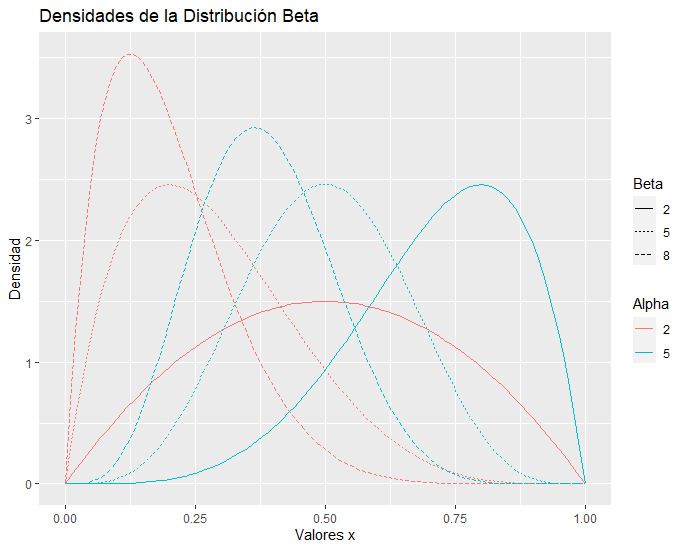
\includegraphics[width=0.45\textwidth]{grafi/dist_beta.jpg}
	\caption{Densidad de la distribución Beta para distintos valores de los parámetros}
	\label{fig:15}
\end{figure}

Vemos que en este caso, nuestra distribución previa y la posteriori pertenecen a la misma familia, en este caso la familia \textit{Beta(a,b)}, a este tipo de distribuciones previas, que para un cierto modelo de los datos mantiene su ''forma'' y cambia los parámetros se les conoce como \textbf{Previa Conjugada} (\cite{hoff_first_2009}).

\subsubsection{Modelo Poisson}

El modelo de Poisson lo usamos para contar la cantidad de ocurrencias de un evento en un determinado tiempo, en economía de la salud podríamos estar interesados en medir la cantidad de episodios epílepticos que tiene un paciente durante un tiempo determinado, entonces, en una muestra de N pacientes, tendremos que $y_1,\ldots,y_N$ la cantidad de episodios epilépticos que tiene cada uno de los pacientes se distribuye $y_i \sim Poisson(\theta)$ que tiene densidad $f_{y_i}(y)=\theta^ye^{-^\theta}/y!$ con $\mathbb{E}(y_i)=\mathbb{V}(y_i)=\theta$ para $y \in \mathbb{N}$.\
Además, sabemos que para $Y=y_1+\ldots+y_N$ con $y_i$ i.i.d $\forall i$ tenemos que $Y\sim Poisson(N\theta)$.\\

En este caso, que $\theta$ no representa una probabilidad, si no la esperanza, la única información que tenemos es que $\theta>0$, se puede demostrar que la \textbf{previa conjugada} para el modelo Poisson es $\theta \sim Gamma(a,b)$ con $a,b>0$ que tiene densidad $f(\theta)=\frac{b^a}{\Gamma{a}}\theta^{a-1}e^{-b\theta}$.\
Luego, aplicando el teorema de Bayes podemos obtener la distribución a posteriori de $\theta$ como una Gamma:\\

\[
\begin{split}
p(\theta|Y) & = \frac{p(Y|\theta)p(\theta)}{p(Y)}\\
& = \left{(}\theta^{a-1}e^{-b\theta}\right{)}\times\left{(}\theta^Ye^{-N\theta}\right{)}\times c(Y,a,b)\\
& = \left{(}\theta^{a+Y-1}e^{-(b+n)\theta}\right{)}\times c(Y,a,b)\\
p(\theta|Y) & \propto \left{(}\theta^{a+Y-1}e^{-(b+N)\theta}\right{)}
\end{split}
\]

Donde $c(Y,a,b)$ es una constante que depende de la distribución de los datos (Y), a, b. Así que deducimos que $\theta|Y\sim Gamma(a + Y, b + N)$ ó también  $\theta|y_1,\ldots,y_N \sim Gamma(a + \sum y_i,b+N)$

\begin{figure}[H]
	\centering
	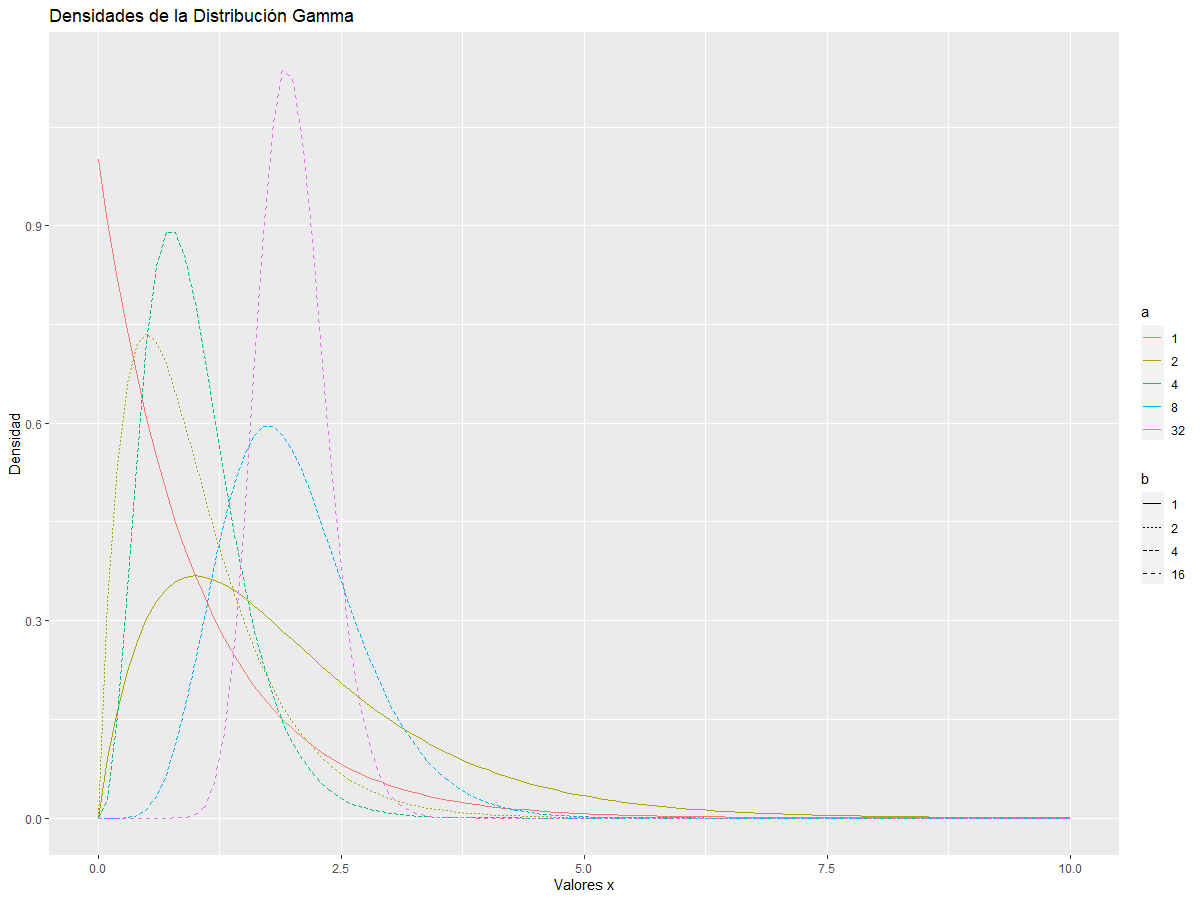
\includegraphics[width=0.45\textwidth]{grafi/dist_gamma.jpg}
	\caption{Densidad de la distribución Gamma para distintos valores de los parámetros}
	\label{fig:16}
\end{figure}

\subsection{Familia Exponencial y Previas conjugadas}

Veamos ahora el caso donde a $y|\phi$ lo podamos modelar con una distribución de la familia exponencial, estas son aquellas que siguen una distribución de la forma: $p(y|\phi)=h(y)c(\phi)e^{\phi t(y)}$ donde $\phi$ es el parámetro desconocido que antes llamábamos $\theta$ y $t(y)$ es un estadístico suficiente, (es decir, una función de \textit{y} que tiene la información necesaria para estimar $\phi$) como por ejemplo $t(y)=\sum y_i$ ó también $t(y)=\bar{y}$.
\

Ylvisaker y Diaconis (1979) estudiaron las previas conjugadas para el modelo exponencial y en particular las de la forma $p(\phi|n_0,t_0) = \kappa(n_0,t_0)c(\psi)^{n_0}e^{n_0 t_0\psi}$ donde $n_0$ y $t_0$ son una forma de expresar la cantidad de ensayos teóricos en la distribución previa  y un estadístico suficiente respectivamente \cite{hoff_first_2009}). Por ejemplo, en el caso de la distribución $Beta(\alpha,\beta)$ podemos expresarlos como $Beta(n_0t_0,n_0(1-t_0))$, con $n_0=\alpha+\beta$ y $t_0=\alpha/(\alpha+\beta)$ que representa la media.
\

De esta forma, cuando estamos frente a una previa que se comporta de acuerdo a lo mostrado anteriormente, y una distribución para los datos que pertenece a la familia exponencial podemos modelar la distribución a posteriori de la forma $p(\phi|y_1,\ldots,y_N) \propto p(\phi|n_0+n,n_0t_0+n\bar{t}(y))$ en donde $\bar{t}(y)$ es la media del estadístico suficiente.

\subsection{Aproximación por Método Monte-Carlo}

Las aproximaciones por el método de Monte-Carlo nos permiten poder calcular la probabilidad de que nuestro parámetro pertenezca a cierto intervalo, o también, como es de nuestro interés para poder modelar la diferencia en la efectividad y los costos entre dos tratamientos, podemos calcular la probabilidad de que $\epsilon_1-\epsilon_0>0$, todo esto mediante simulaciones de la distribución a posteriori (\cite{hoff_first_2009}).
\

Obtener los resultados exactos para $P(\theta \in A|y_1,\ldots,y_N)$ o $P(\epsilon_1-\epsilon_0>0|y_1,\ldots,y_N)$ puede requerir de métodos de cálculos complejos para resolver las integrales. El método Monte-Carlo plantea que una vez obtenida la distribución a posteriori, se hagan \textbf{\textit{S}} simulaciones, que la mayoría de los softwares estadísticos tienen herramientas sencillas para la realización de simulaciones de las distribuciones más conocidas. Por último, por la Ley de Grandes Números, sabemos que si tenemos $\theta^{(1)},\ldots,\theta^{(S)}$ las \textit{S} simulaciones de la distribución a posteriori, entonces $\bar{\theta}=\frac{1}{S}\sum_{s=1}^S\theta^{(s)} \xrightarrow{S \rightarrow \inf} \mathbb{E}(\theta)$.
\

Y aparte, la distribución empírica de $\theta^{(1)},\ldots,\theta^{(S)} \rightarrow p(\theta|y_1,\ldots,y_N)$ por el \textit{Teorema de Glivenko Cantelli}, los que nos permite aproximar $P(\theta \in A|y_1,\ldots,y_N)$ con $\frac{\sum_s \mathbb{I}(\theta^{(s)} \in A)}{S}$\\

\begin{center}
	\textbf{Cadenas de Markov}
\end{center}

En los métodos bayesianos es muy común la utilización del método Monte-Carlo mediante el uso de \textit{Cadenas de Markov}, las Cadenas de Markov, esencialmente es una secuencia de variables aleatorias $Y_0, Y_1,\ldots$ de forma tal que:\\

\[
p(y_{t+1}|y_0,\ldots,y_t)=p(y_{t+1}|y_t)
\]

Es decir, lo que pasa en el momento $t+1$ depende solo de que lo que pasa en el momento inmediato anterior $t$.\
En nuestro análisis, haremos una cantidad suficientemente grande de iteraciones de la Cadena de Markov de la distribución a posteriori de nuestro parámetro y eliminaremos los primeros resultados, para quedarnos con la parte de la Cadena en la que la distribución a posteriori converge. Obteniendo así muchas estimaciones de nuestro parámetro, y mediante los resultados de Monte-Carlo presentados anteriormente determinameremos la distribución a posteriori de nuestro parámetro de interés.\\

Una de las principales características de las Cadenas de Markov es que nos permite incluir previas poco informativas sobre la distribución de los parámetros, o con mucha varianza, ya que en cada paso de la cadena nuestra información previa se va actualizando de forma iterativa. Permitiendo que en un momento \textit{t} suficientemente grande no quede ''rastros'' de nuestra información previa si esta es mala.\\

Una pregunta que puede surgir en esta breve presentación de Cadenas de Markov es ¿cuántas son suficientes iteraciones?, ¿cuántos primeros resultados eliminamos?, ¿cuántas cadenas hacemos?.\
Comunmente, en varios softwares estadísticos se está programado para hacer 4 cadenas de Markov, que usualmente se les asigna distinta previa a cada una, para buscar que todas convergan al mismo resultado. En estas 4 cadenas se suele hacer 2000 iteraciones, y se eliminan las primeras mil (se dice que tiene un \textit{warm-up=1000}).\
Otra pregunta que puede surgir es ¿Qué significa convergencia?, ¿cómo se detecta la convergencia?, para este punto lo que haremos es graficar las estimaciones puntuales de nuestro parámetro en cada una de las iteraciones que no descartamos de nuestras 4 cadenas, y en el gráfico que tiene en el eje de las abscisas el número de iteraciones y en el eje de las ordenadas la estimación puntual para cada iteración de cada una de las 4 cadenas y en el gráfico buscaremos observar... ¡Nada!. Buscaremos que no haya ningún patrón y que además las 4 cadenas se mezclen. A continuación presentaremos dos ejemplos, en el gráfico de arriba de la figura \ref{fig:17} no hay convergencia, mientras que en el gráfico de abajo si hay.\\

\begin{figure}[H]
	\centering
	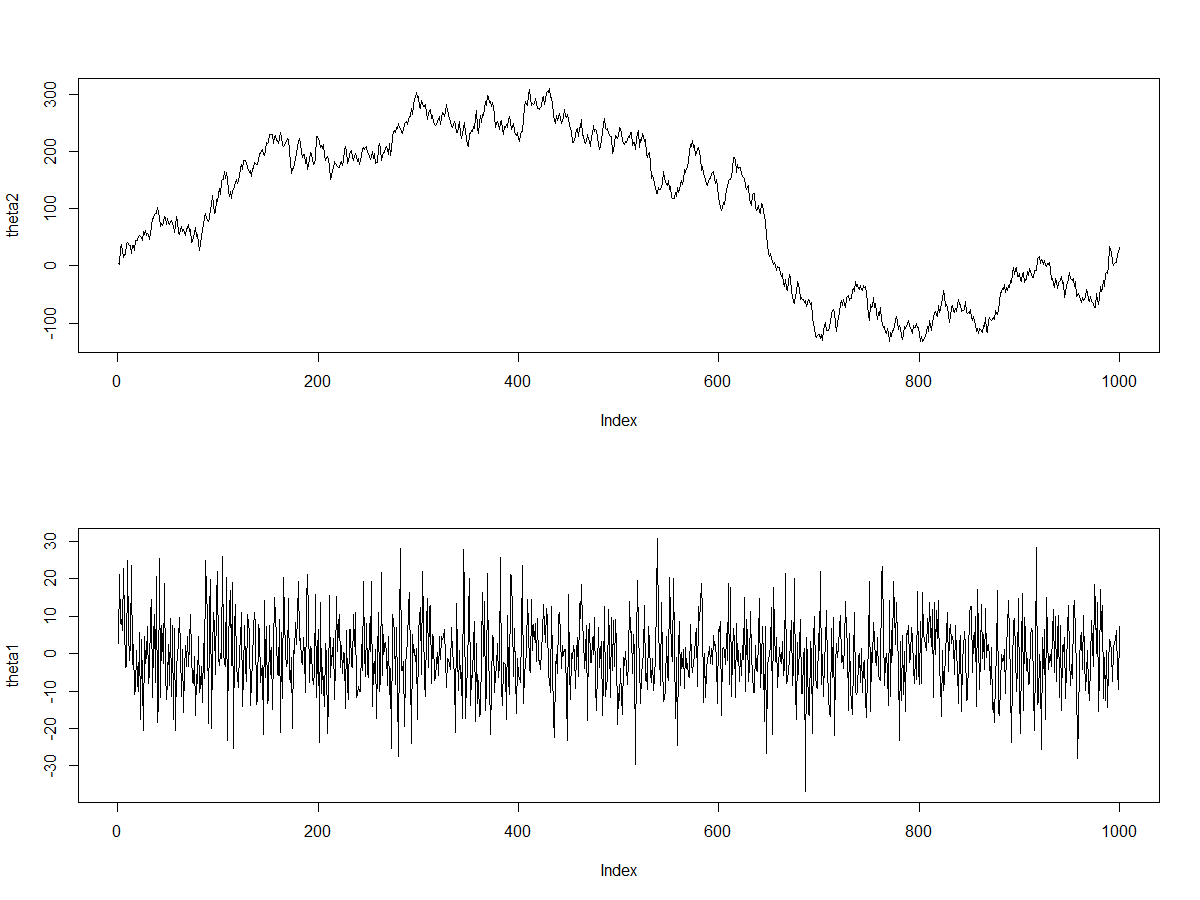
\includegraphics[width=0.45\textwidth]{grafi/conv_y_no_conv.jpg}
	\caption{Convergencia y no convergencia en la estimación de un parámetro}
	\label{fig:17}
\end{figure}

\subsubsection{Algunos Resultados de Aplicar MCMC en R}

Cuando se trabaja con más de una cadena se puede utilizar el $\hat{R}$ como medida de la convergencia, para la estimación del parámetro $\theta$, al poder separar su varianza como entre la varianza dentro de las cadenas y la varianza entre las cadenas, $\hat{R}$ nos da una medida de que tan parecidas son las cadenas, y se suele aceptar como un indicio de convergencia cuando $\hat{R}<1.1$ (\cite{baio_bayesian_2017})\\

\[
\widehat{V}(\theta|y)  = \frac{S-1}{S(W(\theta)} + \frac{1}{S}B(\theta)
\]
\[
\hat{R} = \sqrt{\frac{\widehat{V}(\theta|y)}{W(\theta)}}
\]

Donde $W(\theta)$ y $B(\theta)$ representa la varianza dentro y entre las cadenas, y S es la cantidad de iteraciones

\subsection{Bayes en Evaluación Económica} 

Como se presentó en capítulos anteriores, nuestro principal objetivo es poder hacer una evaluación económica, que contemple los resultados obtenidos, de distintos tratamientos para una misma enfermadad, ó como se presentó en el Análisis Costo-Utilidad o Costo-Beneficio, para distintas enfermedades que tenían prevalencia en una misma población.\

Cuando hacíamos evaluación económica mediante el método de Análisis Costo-Efectividad, tomábamos una decisión según el \textit{ICER} (Ratio Incremental Costo-efectividad) obtenido, donde $ICER_{0,1}=\frac{\gamma_1-\gamma_0}{\epsilon_1-\epsilon_0}$ donde $\epsilon_i$ representava la efectividad del tratamiento \textit{i}, y $\gamma_i$ el costo. Entonces, al comparar el nuevo tratamiento (t=1) con el actual (t=0), el \textit{ICER} nos decía cuánto aumentaba (o disminuía) nuestro costo por cada unidad extra en la efectividad. Con nuestra muestra obteníamos una estimación para el \textit{ICER} ($\widehat{ICER}$). Para lo que precisabamos estimar la diferencia de medias del costo y de la efectividad en ambos tratamientos, por lo que ahora nuestras variables aleatorias son $\Delta_\epsilon$ y $\Delta_\gamma$ que tendrán parámetros desconocidos $\epsilon_0$, $\epsilon_1$, $\gamma_0$ y $\gamma_1$.\
Los métodos bayesianos presentados en esta sección nos dan herramientas para estimar fácilmente $\Delta_\epsilon$ y $\Delta_\gamma$ por separado, para luego de haber hecho el \textit{warm-up} necesario, y asumiendo independencia entre ambas variables, tendremos 1000 valores de ICER, uno para cada pareja $\Delta_\epsilon$, $\Delta_\gamma$ en cada paso de la Cadena de Markov, y aplicaremos los métodos de Monte-Carlo para los 1000 \textit{ICER} obtenidos en cada simulación. 


\section{Bibliografía}

\printbibliography

% \setcitestyle{authoryear,round}


\pagebreak
\thispagestyle{empty}
\begin{center}

\vspace{1.5 cm}
{\Huge Instituto de Estadística} 
\noindent\rule{18cm}{0.4pt}

\vspace{0.5 cm}
\pagestyle{fancy}
{\Huge Serie Documentos de Trabajo}\\
\thispagestyle{empty}
%\noindent\rule{18cm}{0.4pt\includegraphics[width=0.50\textwidth]{grafi/logo_iesta.png}}
\vspace{1.5 cm}

\includegraphics[width=1.00\textwidth]{grafi/logo_inst_80.png}

%\begin{center}
\thispagestyle{empty}
\vspace{4.5 cm}

\begin{flushright}
	\textbf{\large Gonzalo Ramirez 1926, Piso 1, Oficina 23 - C.P. 11200 - Montevideo, Uruguay\\
		Teléfono: (598) 2410 2564\\
		https://iesta.fcea.udelar.edu.uy/\\
		Área Publicaciones\\}	
\end{flushright}

\vspace{1.5 cm}

\large\textbf{Julio, 2023}\\
\vspace{0.5 cm}
\large\textbf{\textnumero 4/23}
\end{center}

\end{document}
 